
\documentclass[letterpaper, 10 pt, conference]{ieeeconf}  % Comment this line out if you need a4paper

%\documentclass[a4paper, 10pt, conference]{ieeeconf}      % Use this line for a4 paper

\IEEEoverridecommandlockouts                              % This command is only needed if 
                                                          % you want to use the \thanks command

\overrideIEEEmargins                                      % Needed to meet printer requirements.

% See the \addtolength command later in the file to balance the column lengths
% on the last page of the document

% The following packages can be found on http:\\www.ctan.org
%\usepackage{graphics} % for pdf, bitmapped graphics files
%\usepackage{epsfig} % for postscript graphics files
%\usepackage{mathptmx} % assumes new font selection scheme installed
%\usepackage{times} % assumes new font selection scheme installed
%\usepackage{amsmath} % assumes amsmath package installed
%\usepackage{amssymb}  % assumes amsmath package installed

\usepackage{macros}


\title{\LARGE \bf
 Deterministic Perturbations For Simultaneous Perturbation Methods Using
 Circulant Matrices.
}



\author{Chandramouli K $^\sharp$, D. Sai Koti Reddy$^\dagger$, Shalabh Bhatnagar$^\ddag$
\thanks{
Department of Computer Science and Automation,
Indian Institute of Science, Bangalore,
E-Mail: $^\sharp$chandramouli.kamanchi@csa.iisc.ernet.in.
$^\dagger$danda.reddy@csa.iisc.ernet.in.
$^\ddag$shalabh@csa.iisc.ernet.in.}
\thanks{$^\star$Supported by Robert Bosch Center for Cyber-Physical Systems, IISc.}
% \thanks{$\ast$ Supported by NSF under Grants CMMI-1434419, CNS-1446665,
% and CMMI-1362303,  by AFOSR under Grant FA9550-15-10050, and
% by the Robert Bosch Centre for Cyber-Physical Systems, IISc.
% }
}



\begin{document}
% 
% 
\maketitle
% \thispagestyle{empty}
% \pagestyle{empty}
% 
% 
%%%%%%%%%%%%%%%%%%%%%%%%%%%%%%%%%%%%%%%%%%%%%%%%%%%%%%%%%%%%%%%%%%%%%%%%%%%%%%%%
\begin{abstract}
We consider the problem of finding optimal parameters under simulation optimization setup.
For a $p$-dimensional parameter optimization, the classical Kiefer-Wolfowitz Finite Difference Stochastic 
Approximation (FDSA) scheme uses $p+1$ or $2p$ simulations of the system feedback for one-sided 
and two-sided gradient estimates respectively.
The dependence on the dimension $p$ makes FDSA impractical for high dimensional problems.
An alternative approach for gradient estimation in high dimensional problems is the 
simultaneous perturbation technique.
%that appears in \cite{spall},\cite{kushcla}.
The main idea in this approach is to estimate the gradient by using only two settings of 
the $p$-dimensional parameter being optimized. 
The two settings of the parameter are obtained by
simultaneously perturbing all the components of the parameter by adding a random 
direction. A drawback of using random directions for the gradient estimate is the very large
or possibly infinite range of these random directions (for e.g. $\pm 1$ symmetric 
Bernoulli perturbations typically used in 1SPSA algorithm has a range of cardinality $2^p$).
In this article we consider deterministic perturbations with a range of cardinality
$p+1$ to improve the convergence of these algorithms. A novel construction of deterministic perturbations 
based on specially chosen circulant matrix is proposed. Convergence analysis of the proposed
algorithms is presented along with numerical experiments. 
\end{abstract}

% Some well known 1st order optimization
% methods used to solve these problems are Simultaneous Perturbation Stochastic Approximation
% (1SPSA) \cite{spall} and Random Directions Stochastic Approximation (1RDSA) \cite{kushcla}
% and their one simulation variants (1s-1SPSA)\cite{spall2},(1s-1RDSA)\cite{bhatnagar-book}.
% While (1SPSA) and (1RDSA) use two simulations per iterate, (1s-1SPSA) and (1s-1RDSA) use
% one simulation per iterate but have high bias.
% All these methods use random perturbations to simulataneously perturb all the parameter 
% components and approximate the gradient. In \cite{bhatnagar2003two} Shalabh et al., introduced
% deterministic perturbations based on Hadamard matrices for 1SPSA, both for one simulation 
% \cite{spall2} and two simulation \cite{spall} variants of the algorithm that empirically 
% perform better than 1SPSA. We introduce deterministic perturbations based on circulant 
% matrices for gradient estimate of 1RDSA and 1s-1RDSA. We prove that 1RDSA and 1s-1RDSA 
% with these perturbations (1RDSA-C,1s-1RDSA-C) converges to the local minimum of the objective 
% funtion of the optimization problem. Further our numerical experiments show that 
% 1RDSA-C (1s-1RDSA-C)
% outperforms 1SPSA (1s-1SPSA) and 1SPSA with Hadamard perturbations,1SPSA-H (1s-1SPSA-H).
% 
% Moreover our circulant matrix based perturbations has the advantage of being useful for
% both one simulation and two simulation variants of the algorithm without any modification.
% Also the results shown to construct the perturbations may be of independent interest.
 
% %%%%%%%%%%%%%%%%%%%%%%%%%%%%%%%%%%%%%%%%%%%%%%%%%%%%%%%%%%%%%%%%%%%%%%%%%%%%%%%%
\section{INTRODUCTION}
Simulation optimization problems frequently arise in engineering disciplines like 
transportation systems, machine learning, service systems, manufacturing etc. 
Practical limitations, lack of model information and the large dimensionality of these 
problems prohibit analytic solution of these problems and simulation is often employed to 
evaluate a system in these disciplines. Hence simulation budget becomes critical and 
one aims to converge to optimal parameters using as few simulations as possible.

To state the problem formally, consider a system where noise-corrupted feedback of the 
system is available i.e., given the system parameter $\theta$ the feedback that is 
available is $h(\theta, \xi)$ where $\xi$ is the noise term inherent in the system, 
pictorially shown in Figure \ref{fig:so}. The objective in these problems is to find a 
parameter vector that gives the optimal expected performance of the system. 
Suppose $J(\theta)=\E_{\xi}[h(\theta, \xi)]$ then $h(\theta, \xi)=J(\theta)+M(\theta,\xi)$ 
where $M(\theta,\xi)=h(\theta, \xi)-\E_{\xi}[h(\theta, \xi)]$ is a mean zero term. Hence, one 
needs to solve the following optimization problem:
\begin{align}
\mbox{Find } \theta^* = \arg\min_{\theta \in \R^p} J(\theta). \label{eq:pb}
\end{align}
Analogous to deterministic optimization problems, where explicit analytic gradient of the 
objective function is available, a solution approach could be to devise an algorithm that 
mimics the familiar gradient descent algorithm. However in our setting only noise corrupted 
samples of the objective are available. So one essentially needs to estimate the gradient 
of the objective function using simulation samples.

This adaptive system optimization framework has its roots in the work by 
Robbins and Monro \cite{robbins1951} and Kiefer and Wolfowitz \cite{kiefer1952}. 
The work by Kiefer and Wolfowitz uses stochastic approximation framework by 
Robbins and Monro to optimize an objective using noisy samples. In their work
Kiefer and Wolfowitz \cite{kiefer1952} use 
one-sided or two-sided approximation of the gradient. 
This method has the drawback of using $p+1$ simulations for one-sided approximation and
$2p$ simulations for two-sided approximation of the gradient for a 
$p$-dimensional problem. Later works \cite{kushcla},\cite{spall} have replaced the 
gradient approximation using finite differences with random perturbations.

Simultaneous perturbation is a useful technique to estimate the gradient from the function 
samples, especially in high dimensional problems - see \cite{bhatnagar-book},
\cite{spallbook} for a comprehensive treatment of this subject matter.
The first-order Simultaneous Perturbation Stochastic Approximation algorithm for 
simulation optimization, henceforth referred to as 1SPSA-2R, was 
proposed in \cite{spall}. 1SPSA-2R uses two simulations per iteration and random 
perturbations to perturb the parameter vector. 
A one measurement variant of \cite{spall} is proposed in \cite{spall2} which we refer here
as 1SPSA-1R.
A closely related algorithm is the first-order Random Directions 
Stochastic Approximation henceforth referred to as 1RDSA-2R that appears in
\cite[pp.~58-60]{kushcla}.
The algorithm 1RDSA-2R differs from 1SPSA-2R, both in the construction as well as 
convergence analysis and performs poorly compared to 1SPSA-2R, see 
\cite{chin1997comparative} for a detailed comparative study. 

To enhance the performance of 1SPSA-2R and 1SPSA-1R, \cite{bhatnagar2003two}
proposed deterministic perturbations based on Hadamard matrices.
We refer here the variants of 1SPSA-2R and 1SPSA-1R that use Hadamard perturbations as
1SPSA-2H and 1SPSA-1H. Analogous to their work we propose deterministic perturbations
for 1RDSA-2R and its  one simulation variant (referred as 1RDSA-1R here) based on a
specially chosen circulant matrix.
\tikzstyle{block} = [draw, fill=white, rectangle,
   minimum height=3em, minimum width=6em]
\tikzstyle{sum} = [draw, fill=white, circle, node distance=1cm]
\tikzstyle{input} = [coordinate]
\tikzstyle{output} = [coordinate]
\tikzstyle{pinstyle} = [pin edge={to-,thin,black}]
\begin{figure}[t]
    \centering
\scalebox{0.8}{\begin{tikzpicture}[auto, node distance=2cm,>=latex']
% We start by placing the blocks
\node (theta) {$\boldsymbol{\theta}$};
\node [block, fill=blue!20,right=0.6cm of theta,align=center] (sample) {\makecell{\textbf{System simulator}}}; 
\node [right=0.6cm of sample] (end) {$\boldsymbol{{h(\theta, \xi)}}$};
\node [ above right= 0.6cm of end] (bias){\textbf{feedback}};
\draw [->] (theta) --  (sample);
\draw [->] (sample) -- (end);
\path [darkgreen,->] (bias) edge [bend left] (end);
\end{tikzpicture}}
\caption{Simulation Optimization Model}
\label{fig:so}
\end{figure}
\section{MOTIVATION}
Here we motivate the necessary conditions that deterministic perturbations should satisfy.
Analogous properties for Hadamard matrix based perturbations are well motivated in 
\cite{bhatnagar-book}.
Both 1SPSA-2R and 1RDSA-2R iteratively update the parameter vector and a typical update step
is of the following form:
\begin{align}
\label{eq:grad-descent}
\theta_{n+1} = \theta_n - a_n \widehat\nabla J(\theta_n), 
\end{align}
where $a_n$ is the step-size that satisfies standard stochastic approximation 
conditions (see (A2) in section \ref{sec:convergenceresults}) and $\widehat\nabla 
J(\theta)$ is an estimate of the gradient of the objective function $J$.
Thus, \eqref{eq:grad-descent} can be considered as 
the stochastic version of the well-known gradient descent method for optimization. 
% Now consider the Taylor series expansion of $J(\theta_n+\delta_nd_n)$ around
% $\theta_n$, we have
% \begin{equation} \label{eq:pTaylor}
% J(\theta_n+\delta_nd_n)=
% J(\theta_n)+\delta_nd_n^T \nabla J(\theta_n)+o(\delta_n).
% \end{equation}
% Similarly, an expansion of $J(\theta_n-\delta_n d_n)$ around $\theta_n$ gives
% \begin{equation} \label{eq:nTaylor}
% J(\theta_n-\delta_n d_n)=
% J(\theta_n)-\delta_n d_n^T \nabla J(\theta_n)+o(\delta_n).
% \end{equation}
% From \eqref{eq:pTaylor} and \eqref{eq:nTaylor}, we have
% \begin{align}\label{eq:Taylor}
% &\frac{J(\theta_n+\delta_n d_n)-J(\theta_n-\delta_n d_n)}{2\delta_n}d_n
% - \nabla J(\theta_n) \\
% &= (d_nd_n^T-I)\nabla J(\theta_n)+o(\delta_n).
% \end{align}
Now consider the Taylor series expansion of $J(\theta_n \pm \delta_nd_n)$ around
$\theta_n$, we have
 \begin{equation} \label{eq:pmTaylor}
 J(\theta_n \pm \delta_nd_n)=
 J(\theta_n) \pm \delta_nd_n^T \nabla J(\theta_n)+o(\delta_n).
\end{equation}
From \eqref{eq:pmTaylor}, we have
\begin{align}\label{eq:Taylor}
&\frac{J(\theta_n+\delta_n d_n)-J(\theta_n-\delta_n d_n)}{2\delta_n}d_n
 - \nabla J(\theta_n) \\
&= (d_nd_n^T-I)\nabla J(\theta_n)+o(\delta_n).
\end{align}
Note that $(d_nd_n^T-I)\nabla J(\theta_n)$ constitutes the bias in the
gradient estimate and
from the assumption (A3) in section \ref{sec:convergenceresults}
\begin{equation}\label{eq:2sidedbias}
\mathbb{E}\Big{[}(d_nd_n^T-I)\nabla J(\theta_n)\Big{|}\theta_n\Big{]}=0.
\end{equation}
In the case of a one-simulation algorithm with parameter $\theta_n+\delta_n d_n$,
a similar Taylor series expansion gives
\begin{align}\label{eq:1sided}
&\frac{J(\theta_n+\delta_n d_n)}{\delta_n}d_n
- \nabla J(\theta_n) \\
&=\frac{J(\theta_n)}{\delta_n}d_n
+(d_nd_n^T-I)\nabla J(\theta_n)+O(\delta_n).
\end{align}
One expects the following to hold in addition to \eqref{eq:2sidedbias} in the case of 
random perturbations for one simulation algorithms:
\begin{equation}\label{eq:1sidedbias}
\mathbb{E}\Big{[}\frac{J(\theta_n)}{\delta_n}d_n\Big{|}\theta_n\Big{]}=0. 
\end{equation}
Notice that \eqref{eq:2sidedbias} and \eqref{eq:1sidedbias} are achieved asymptotically 
for a random perturbation direction $d_n$, for example with $\pm 1$ symmetric Bernoulli 
components, $d_n$ has to cycle through $2^p$ possible vectors in the range to achieve bias 
cancellation. Clearly one is motivated to look for perturbations that satisfy similar 
properties and have a smaller cycle length for faster bias cancellation and thereby 
improve the performance of the algorithm. 
Analogous to \eqref{eq:2sidedbias} and \eqref{eq:1sidedbias} we expect deterministic sequence 
of perturbations to satisfy the following properties:
\begin{enumerate}[label=\textbf{(P\arabic*)}]
  \item Let $D_n:=d_nd_n^T-I.$ For any $s \in \mathbb{N}$ there exists a 
  $P \in \mathbb{N}$ such that $\sum\limits_{n=s+1}^{s+P}D_n=0$ and,
  \item  $\sum\limits_{n=s+1}^{s+P}d_n=0.$
\end{enumerate}
In the following sections we construct deterministic perturbations which satisfy (P1) and (P2)
and provide convergence results for the resulting 1RDSA-2C and 1RDSA-1C algorithms.

The rest of the paper is organized as follows: In section \ref{sec:algo}, we
describe the various ingredients in algorithm \ref{alg:structure} and the construction
of perturbations $d_n$.
In section \ref{sec:convergenceresults}, 
we present the convergence results for 1RDSA-2C and 1RDSA-1C algorithms.
In section~\ref{sec:expts}, we present the results from numerical experiments and finally, 
in section~\ref{sec:conclusions}, we provide the concluding remarks.
\section{STRUCTURE OF THE ALGORITHM}
\label{sec:algo}
\begin{algorithm}[t]
\begin{algorithmic}
\State {\bf Input:}
\begin{itemize}
 \item $\theta_0 \in \mathbb{R}^p,$ initial parameter vector;
 \item $\delta_n, n \geq 0,$ a sequence to approximate gradient;
 \item Matrix of perturbations $$Q=\sqrt{p+1}[H^{-1/2},-H^{-1/2}u],$$ 
 with $u=[1,1,\cdots,1]^T;$
 \item noisy measurement of cost objective $J$;
 \item $a_n, n \geq 0,$ step-size sequence satisfying assumption \ref{stepsizes} of 
 section \ref{sec:convergenceresults};
\end{itemize}
\For{$n = 1,2,\ldots n_{\text{end}}$}	
	\State Let $d_n$ be mod$(n,p+1)^{\text{th}}$ column of $Q$. 
	\State Update the parameter as follows:
  \begin{equation}
  \theta_{n+1}=\theta_n-a_n \widehat\nabla J(\theta_n), \label{eq:algo}
  \end{equation}
where $\widehat\nabla J(\theta_n)$ is chosen according to \eqref{eq:grad-twosided} 
or \eqref{eq:grad-onesided}. 
\EndFor
\State {\bf Return} $\theta_{n_{\text{end}}}.$
\end{algorithmic}
\caption{Basic structure of 1RDSA-2C and 1RDSA-1C algorithms.}
\label{alg:structure}
\end{algorithm}
Algorithm \ref{alg:structure} presents the basic structure of 
1RDSA-2C and 1RDSA-1C. We describe the individual 
components of algorithm \ref{alg:structure} below.
\subsection{Deterministic Pertubations}
Let $\delta_n, n\geq 0$ denote a sequence of diminishing positive real numbers satisfying 
assumption (A2) in section \ref{sec:convergenceresults} and 
$d_n = (d_n^1,\ldots,d_n^p)\tr$ denote $(p+1)$ mod $n$ column of $Q.$
where $Q$ is constructed as follows. 
Let $H$ be the $p \times p$ dimensional matrix defined as:
\begin{equation}\label{eq:H}
H = \left[\begin{array}{cccc}
2 \ 1 \ 1 \cdots 1\\ 
1 \ 2 \ 1 \cdots 1 \\
\vdots \ \vdots \ \vdots \ \vdots\\
1 \ 1 \ 1 \cdots 2
\end{array}\right].
\end{equation}
Observe that $H=I+uu^T$, where $u=[1,1,\cdots,1]^T$, is a positive definite matrix. Hence $H^{-1/2}$ is well defined.
Define $p\times (p+1)$ matrix $Q$ as $Q=\sqrt{p+1}[H^{-1/2},-H^{-1/2}u].$ The columns of
$Q$ are used as perturbations $d_n.$
\subsection{Gradient estimation}
Let $y_{n}^{+}$, $y_{n}^{-}$  be defined as below.
$y_{n}^{+} = J(\theta_n+\delta_n d_n) + M_{n}^{+}$ and 
$y_{n}^{-} = J(\theta_n-\delta_n d_n) + M_{n}^{-}$,
where the noise terms $M_{n}^{+}, M_{n}^{-}$ satisfy $\E\left[\left.M_{n}^{+}- 
M_{n}^{-}\right| \F_n\right] = 0$ with $\F_n = \sigma(\theta_m, m\le n)$ 
denoting the underlying sigma-field. 
The estimate of the gradient $\nabla J(\theta_n)$ is given by
\begin{align}
\label{eq:grad-twosided}
\widehat\nabla J(\theta_n)=
\left[\dfrac{(y_{n}^{+} - y_{n}^{-})d_n}{2\delta_n}\right] \text{ for 1RDSA-2C}
\end{align}
\begin{align}
\label{eq:grad-onesided}
\widehat\nabla J(\theta_n)=
\left[\dfrac{(y_{n}^{+})d_n}{\delta_n}\right] \text{ for 1RDSA-1C}
\end{align}
Observe that while 1RDSA-2C algorithm uses two function samples $y_{n}^{+}$ and $y_{n}^{-}$ 
at $\theta_n+\delta_n d_n$ and $\theta_n - \delta_n d_n$, 1RDSA-1C algorithm 
uses only one function sample $y_{n}^{+}$ at $\theta_n+\delta_n d_n$.
\section{CONVERGENCE ANALYSIS}
\label{sec:convergenceresults}
We make the same assumptions as those used in the analysis of \cite{spall}, with a 
few minor alterations. The assumptions are listed below.

\begin{enumerate}[label= \textbf{A\arabic*}.]
 \item The map $J:\mathbb{R}^p \rightarrow \mathbb{R}$ is Lipschitz continuous and 
 is differentiable with bounded second order derivatives. Further, 
 the map $L:\mathbb{R}^p \rightarrow \mathbb{R}$ defined as 
 $L(\theta)=-\nabla J(\theta)$ is Lipschitz continuous.
 \item The step-size sequences $a_n, \delta_n >0, \forall n $  satisfy
 \begin{equation*}\label{stepsizes}
 a_n,\delta_n \text{ as } n \rightarrow \infty, \sum_na_n=\infty,
 \sum_n \Big{(}\frac{a_n}{\delta_n}\Big{)}^2<\infty.
 \end{equation*}
 Further, $\frac{a_j}{a_n}\rightarrow 1$ as $n\rightarrow \infty$, for all
 $j \in \{n,n+1,\cdots,n+M\}$ for any given $M>0$ and $b_n=\frac{a_n}{\delta_n}$ is 
 such that $\frac{b_j}{b_n}\rightarrow 1$ as $n\rightarrow \infty$, for all
 $j \in \{n,n+1,n+2,\cdots,n+M\}.$

 \item The random vectors $d_n$, $n\geq0$ are mutually independent and identically
 distributed. Moreover $\mathbb{E}[d_nd_n^T]=I.$
 
 \item The iterates $\theta_n$ remain uniformly bounded almost surely, i.e,
 $$ \sup_n\|\theta_n\|<\infty, a.s.$$

 \item The set $G$ containing the globally asymptotically stable equilibria of the 
 ODE $\dot{\theta}(t)=-\nabla J(\theta(t)) $ (i.e., the local minima of $J$)
 is a compact subset of $\mathbb{R}^N.$
 
 \item The sequences $(M_{n}^{+},\F_n),(M_{n}^{-},\F_n), n\geq0 $ form martingale difference sequences.
 Further, $(M_{n}^{+},M_{n}^{-},n\geq0)$ are square integrable random variables satisfying
 $$\E[\|M_{n+1}^{\pm}\|^2|f_n]\leq K(1+\|\theta_n\|^2) \text{ a.s., } \forall n\geq0,$$
 for a given constant $K \geq 0$
 
\end{enumerate}
The following lemma is useful in obtaining the negative square root of $H$ i.e., 
$H^{-1/2}$. Also note that it takes only $O(p)$ operations to compute $H^{-1/2}$
using the lemma and circulant structure of $H^{-1/2}$.
\begin{lemma}
 \label{lemma: gen Sherman-Morisson}
Let $I$ be a $p \times p$ identity matrix and $u = 
\left[
 \begin{array}{cccc}
 1 \\ 1 \\  \vdots \\ 1 
\end{array} \right]$ be a $p \times 1$ all ones vector then
$$ (I+uu^T)^{-1/2}= I-\frac{uu^T}{p}+\frac{uu^T}{p\sqrt{(1+p)}}.$$
\end{lemma}

\begin{proof}
It is enough to show that
$$(I+uu^T)\Bigg{[}I-\frac{uu^T}{p}+\frac{uu^T}{p\sqrt{(1+p)}}\Bigg{]}^2=I.$$
Using $\|u\|^2=u^Tu=p$ we have
\begin{align*}
 & (I+uu^T)\Bigg{[}I-\frac{uu^T}{p}+\frac{uu^T}{p\sqrt{(1+p)}}\Bigg{]}^2\\
 &= (I+uu^T)\Bigg{[}I-\frac{uu^T}{p}+\frac{uu^T}{p\sqrt{(1+p)}}\\
 &-\frac{uu^T}{p}+\frac{uu^T}{p}-\frac{uu^T}{p\sqrt{(1+p)}}\\
 &+\frac{uu^T}{p\sqrt{(1+p)}}-\frac{uu^T}{p\sqrt{(1+p)}}+\frac{uu^T}{p(1+p)}\Bigg{]}\\
 &=(I+uu^T)\Bigg{[}I-uu^T(\frac{1}{p}-\frac{1}{p(1+p)})\Bigg{]}\\
 &=(I+uu^T)\Bigg{[}I-\frac{uu^T}{1+p}\Bigg{]}\\
 &=I+uu^T-\frac{uu^T}{1+p}-\frac{puu^T}{1+p}\\
 &=I
\end{align*}
proving the lemma.
\end{proof}
As defined earlier let \begin{equation*} H = \left[\begin{array}{cccc}
2 \ 1 \ 1 \cdots 1\\ 
1 \ 2 \ 1 \cdots 1 \\
\vdots \ \vdots \ \vdots \ \vdots\\
1 \ 1 \ 1 \cdots 2
\end{array}\right]
\end{equation*}
and $Q=\sqrt{p+1}[H^{-1/2},-H^{-1/2}u].$
Let the perturbations $d_n$ be the columns of Q. 
\begin{lemma}
 The perturbations $d_n$ chosen as columns of Q satisfy properties P1 and P2.
\end{lemma}
\begin{proof}
 Let $P=p+1$. Observe that as $n$ goes through one cycle from $1$ to $p+1$ we have
 $\sum\limits_{n=1}^{p+1}d_nd_n^T=QQ^T$ and 
 $\sum\limits_{n=1}^{p+1}d_n= Q\left[\begin{array}{cccc}
 u\\ 1 \end{array}\right]$.
 Now it is enough to show that
 $\sum\limits_{n=s+1}^{s+P}D_n=0$ and 
 $\sum\limits_{n=s+1}^{s+P}d_n= 0$ i.e., 
 $Q\left[\begin{array}{cccc}
 u\\ 1 \end{array}\right]=0 \text{ for the choice } s=0.$
 Consider
 \begin{align*}
 & \sum_{n=0}^{P}D_n\\
 & =\sum_{n=1}^{P}(d_nd_n^T-I)\\
 & =\sum_{n=1}^{P}(d_nd_n^T)-(p+1)I\\
 & =QQ^T-(p+1)I\\
 & =(p+1)([H^{-1/2},-H^{-1/2}u][H^{-1/2},-H^{-1/2}u]^T-I)\\
 & =(p+1)([H^{-1}+H^{-1/2}uu^TH^{-1/2}]-I)\\
 & =(p+1)(H^{-1/2}(I+uu^T)H^{-1/2}-I)\\
 & =(p+1)(H^{-1/2}(H)H^{-1/2}-I)\\
 & = 0.
 \end{align*}
 In addition,
 \begin{align*}
 Q\left[\begin{array}{cccc}
 u\\ 1 \end{array}\right]
 & = \sqrt{p+1}([H^{-1/2},-H^{-1/2}u]) \left[\begin{array}{cccc}
 u\\ 1 \end{array}\right]\\
 & = \sqrt{p+1}(H^{-1/2}u-H^{-1/2}u)\\
 & = 0
 \end{align*}
proving the lemma.
\end{proof}
\begin{lemma}
 Given any fixed integer $P>0$, $\|\theta_{m+k}-\theta_{m}\| \rightarrow 0$ $w.p.1,$ as
 $m \rightarrow \infty,$ for all $k \in {1,\cdots, P}$
\end{lemma}
\begin{proof}
 Fix a $k \in \{1,\cdots,P \}.$ Now
 \begin{align*}
 \begin{split}
 \theta_{n+k} = \theta_n & -\sum_{j=n}^{n+k-1}a_j\Bigg{(}\frac{J(\theta_j+\delta_j d_j)-J(\theta_j-\delta_j d_j)}{2\delta_j}\Bigg{)}d_j \\ 
  &-\sum_{j=n}^{n+k-1}a_jM_{j+1}
 \end{split}
 \end{align*}
 Thus,
 \begin{align*}
 \begin{split}
 \|\theta_{n+k}-\theta_n\| &\leq \sum_{j=n}^{n+k-1}a_j\Bigg{|}\Bigg{(}\frac{J(\theta_j+\delta_{j} d_j)-J(\theta_j-\delta_{j} d_j)}{2\delta_j}\Bigg{)}\Bigg{|}d_j\\
 &-\sum_{j=n}^{n+k-1}a_jM_{j+1}
\end{split}
 \end{align*}
Now clearly,
$$N_n=\sum_{j=0}^{n-1}a_jM_{j+1}, n\geq1,$$
forms a martingale sequence.
Further, from the assumption A6 we have,
\begin{align*}
& \sum_{m=0}^{n}\mathbb{E}[\|N_{m+1}-N_{m}\|^2|\mathcal{F}_{m}] \\
& =\sum_{m=0}^{n}\mathbb{E}[a_{m}^2\|M_{m+1}\|^2|\mathcal{F}_{m}]\\
& \leq \sum_{m=0}^{n}a_{m}^2K(1+\|\theta_n\|^2)
\end{align*}
From the assumption A4 the quadratic variation process of $N_n,n\geq0$ converges 
almost surely. Hence by the martingale convergence theorem, it follows that 
$N_n, n\geq0$ converges almost surely. Hence
$\|\sum\limits_{j=n}^{n+k-1}a_jM_{j+1}\|\rightarrow 0$ almost surely as $n\rightarrow \infty.$
Moreover
\begin{align*}
&\Big{\|}\Big{(}J(\theta_j+\delta_j d_j)-J(\theta_j-\delta_j d_j)\Big{)}d_j\Big{\|} \\
& \leq \Big{|}\Big{(}J(\theta_j+\delta_j d_j)-J(\theta_j-\delta_j d_j)\Big{)}\Big{|}\|d_j\|\\
& \leq C \Big{(}|J(\theta_j+\delta_j d_j)|+|J(\theta_j-\delta_j d_j)|\Big{)},
\end{align*}
since $\|d_j\|\leq C, \forall j \geq0.$
Note that
\begin{align*}
|J(\theta_j+\delta_j d_j)|-|J(0)| & \leq|J(\theta_j+\delta_j d_j)-J(0)| \\
& \leq \hat{B} \|\theta_j+\delta_j d_j\|,
\end{align*}
where $\hat{B}$ is the Lipschitz constant of the function $J(.).$ Hence,
$$|J(\theta_j+\delta_j d_j)|\leq \tilde{B}(1+\|\theta_j+\delta_j d_j\|),$$
for $\tilde{B}=$max$(|J(0)|,\hat{B}).$ Similarly,
$$|J(\theta_j-\delta_j d_j)|\leq \tilde{B}(1+\|\theta_j-\delta_j d_j\|).$$
From assumption A4 and triangle inequality, it follows that
$$\sup_j\Big{\|}\Big{(}J(\theta_j+\delta_j d_j)-J(\theta_j-\delta_j d_j)\Big{)}d_j\Big{\|}\leq \tilde{K}<\infty,$$
for some $\tilde{K}>0.$ Thus,
\begin{align*}
& \|\theta_{n+k}-\theta_n\| \leq \tilde{K}\sum_{j=n}^{n+k-1}\frac{a_j}{\delta_j}+\|\sum_{j=n}^{n+k-1}a_jM_{j+1}\|\\
& \rightarrow 0 \text{ a.s. with } n \rightarrow \infty.
\end{align*}
proving the lemma.
\end{proof}
\begin{lemma}
$\text{ For any } m \geq0,$\\
$$\Big{\|}\sum_{n=m}^{m+P-1}\frac{a_n}{a_m}D_n\nabla J(\theta_n)\Big{\|}\rightarrow 0 \text{ and }$$
$$\Big{\|}\sum_{n=m}^{m+P-1}\frac{b_n}{b_m}d_nJ(\theta_n)\Big{\|}\rightarrow 0,$$
$\text{almost surely, as } m \rightarrow \infty.$
\end{lemma}
\begin{proof}
 From lemma 3, it can be seen that 
 $\|\theta_{m+s}-\theta_{m}\|\rightarrow 0$ as $m\rightarrow \infty,$
 for all $s=1,\cdots,P.$ Also from assumption A1, we have
 $\|\nabla J(\theta_{m+s})-\nabla J(\theta_{m})\|\rightarrow 0$ as $m\rightarrow \infty,$
 for all $s=1,\cdots,P.$ Now from lemma 2 $\sum\limits_{n=m}^{m+P-1}D_n=0$ $\forall m\geq0.$
 Thus, 
 \begin{align*}
  &\Big{\|}\sum_{n=m}^{m+P-1}\frac{a_n}{a_m}D_n\nabla J(\theta_n)\Big{\|}\\
  & = \Big{\|}\sum_{n=m+1}^{m+P-1}\frac{a_n}{a_m}D_n\nabla J(\theta_n)
  +D_{m}\nabla J(\theta_{m})\Big{\|}\\
  &=\Big{\|}\sum_{n=m+1}^{m+P-1}\frac{a_n}{a_m}D_n \nabla J(\theta_n)
     -\sum_{n=m+1}^{m+P-1}D_n\nabla J(\theta_{m})\Big{\|}\\
  &=\Big{\|}\sum_{n=m+1}^{m+P-1}D_n\Big{(}\frac{a_n}{a_m}\nabla J(\theta_n)
  -\nabla J(\theta_{m})\Big{)}\Big{\|}\\
  &\leq \bar{K}\sum_{n=m+1}^{m+P-1}\Big{\|}\Big{(}\frac{a_n}{a_m}\nabla J(\theta_n)
  -\nabla J(\theta_{m})\Big{)}\Big{\|}\\
  &=\bar{K}\sum_{n=m+1}^{m+P-1}\Bigg{\|}\Big{(}\frac{a_n}{a_m}-1\Big{)}\nabla J(\theta_n)
   +\Big{(}\nabla J(\theta_n)-\nabla J(\theta_{m})\Big{)}\Bigg{\|}\\
  &\leq \bar{K}\sum_{n=m+1}^{m+P-1}\Bigg{\|}\Big{(}\frac{a_n}{a_m}-1\Big{)}\nabla J(\theta_n)\Bigg{\|}
  +\Bigg{\|}\nabla J(\theta_n)-\nabla J(\theta_{m})\Bigg{\|}\\
  &\text{ The claim now follows as a consequence of the}\\
  &\text{ assumptions A1 and A2.}\\
  &\text{ Now observe that $\|J(\theta_{m+k})-J(\theta_{m})\|\rightarrow 0$ as}\\
  &\text{$m\rightarrow \infty, $ for all $k \in \{1,\cdots,P\}.$ }\\
  &\text{ as a consequence of lemma3 and A1,}\\
  & \Bigg{\|}\sum_{n=m}^{m+P-1}\frac{b_n}{b_m}d_n J(\theta_n)\Bigg{\|}\\
  & =\Bigg{\|}\sum_{n=m+1}^{m+P-1}\frac{b_n}{b_m}d_n J(\theta_n)+d_m J(\theta_{m})\Bigg{\|}\\
  & =\Bigg{\|}\sum_{n=m+1}^{m+P-1}\frac{b_n}{b_m}d_n J(\theta_n)-\sum_{n=m+1}^{m+P-1}d_n J(\theta_{m})\Bigg{\|}\\
  & =\Bigg{\|}\sum_{n=m+1}^{m+P-1}d_n\Big{(}\frac{b_n}{b_m}J(\theta_n)-J(\theta_{m})\Big{)}\Bigg{\|}\\
  & \leq \sum_{n=m+1}^{m+P-1}\Big{\|}d_n\Big{(}\frac{b_n}{b_m}J(\theta_n)-J(\theta_{m})\Big{)}\Big{\|}\\
  & \leq \bar{\bar{K}}\sum_{n=m+1}^{m+P-1}\Big{\|}\Big{(}\frac{b_n}{b_m}J(\theta_n)-J(\theta_{m})\Big{)}\Big{\|}\\
  & =\bar{\bar{K}}\sum_{n=m+1}^{m+P-1} \Bigg{\|}\Big{(}\frac{b_n}{b_m}-1\Big{)} J(\theta_n)
  +\Big{(} J(\theta_n)-J(\theta_{m})\Big{)}\Bigg{\|}\\
  &\leq \bar{\bar{K}}\sum_{n=m+1}^{m+P-1}\Bigg{\|}\Big{(}\frac{b_n}{b_m}-1\Big{)} J(\theta_n)\Bigg{\|}
  +\Bigg{\|}\Big{(} J(\theta_n)- J(\theta_{m})\Big{)}\Bigg{\|}\\
\end{align*}
 The claim now follows as a consequence of the assumptions A1 and A2.
 \end{proof}
\begin{theorem}
 $\theta_n, n\geq0$ obtained from 1RDSA-2C satisfy $\theta_n \rightarrow G$
 almost surely.
\end{theorem}
\begin{proof}
 Note that
 \begin{align*}
  \begin{split}
  & \theta_{n+P} = \theta_n- \\ 
  &\sum_{l=n}^{n+P-1}a_l\Big{(}\frac{J(\theta_l+\delta_l d_l)-J(\theta_l-\delta_l d_l)}{2\delta_l}d_j+M_{l+1}\Big{)}
 \end{split}
 \end{align*}
It follows that
 \begin{align*}
  \begin{split}
  & \theta_{n+P} = \theta_n- \sum_{l=n}^{n+P-1}a_l\nabla J(\theta_l)\\ 
  & -\sum_{l=n}^{n+P-1}a_l(d_ld_l^T-I)\nabla J(\theta_l)\\
  & -\sum_{l=n}^{n+P-1}a_lo(\delta_l)
  -\sum_{l=n}^{n+P-1}a_lM_{l+1}
 \end{split}
 \end{align*}
Now the third term on the RHS can be written as
$$a_n\sum_{l=n}^{n+P-1}\frac{a_l}{a_n}D_{l}\nabla J(\theta_l)=a_n\xi_{n},$$
where $\xi_{n}=o(1)$ from lemma 4.
Thus, the algorithm is asymptotically analogous to
$$\theta_{n+1}=\theta_n-a_n(\nabla J(\theta_n)+o(\delta)+M_{n+1}).$$
Hence from chapter 2 of \cite{borkar2008stochastic} we have that $\theta_n$ converge to
local minima of the function $J.$
\end{proof}

\begin{theorem}
  $\theta_n, n\geq0$ obtained from 1RDSA-1C satisfy $\theta_n \rightarrow G$
 almost surely.
\end{theorem}
\begin{proof}
Note that
 \begin{align*}
 \theta_{n+P} = \theta_n-\sum_{l=n}^{n+P-1}a_l\Big{(}\frac{J(\theta_l+\delta_l d_l)}{2\delta_l}\Big{)}d_l-\sum_{l=n}^{n+P-1}a_lM_{l+1}
 \end{align*} 
It follows that
 \begin{align*}
  \begin{split}
  & \theta_{n+P} = \theta_n- \sum_{l=n}^{n+P-1}a_l\nabla J(\theta_l)\\ 
  & -\sum_{l=n}^{n+P-1}a_l\frac{J(\theta_l)}{\delta_l}d_l-\sum_{l=n}^{n+P-1}a_l(d_ld_l^T-I)\nabla J(\theta_l)\\
  & -\sum_{l=n}^{n+P-1}a_lO(\delta_l)
  -\sum_{l=n}^{n+P-1}a_lM_{l+1}
 \end{split}
 \end{align*}
 Now we observe that
 \begin{align*}
 & \sum_{l=n}^{n+P-1}a_l\frac{J(\theta_l)}{\delta_l}d_l= \sum_{l=n}^{n+P-1} b_{l}J(\theta_l)d_l\\
 & = b_n\sum_{l=n}^{n+P-1}\frac{b_l}{b_n}\frac{J(\theta_l)}{\delta_l}d_l=b_n\xi^{1}_{n},
 \end{align*}
 where $\xi^{1}_{n}=o(1)$ by lemma 4. Similarly
 $$\sum_{l=n}^{n+P-1}a_l(d_ld_l^T-I)\nabla J(\theta_l)=a_n\xi^{2}_{n},$$
 with $\xi^{2}_{n}=o(1)$ by lemma 4.
 The rest follows as explained in Theorem 5.
\end{proof}

\section{SIMULATION EXPERIMENTS}
\label{sec:expts}
\subsection{Implementation}
We compare the performance of 1SPSA-2R, 1SPSA-2H and 1RDSA-2C in the case of 
two simulation algorithms. In the case of one simulation algorithms we compare the 
performance of 1SPSA-1R, 1SPSA-1H and 1RDSA-1C. 
We chose i.i.d Bernoulli $\pm 1$-valued perturbations for 1SPSA-2R and 1SPSA-1R.
\footnote{The implementation is available at 
\url{https://github.com/cs1070166/1RDSA-2Cand1RDSA-1C/}}

For the empirical evaluations, 
we use the following two loss functions in $p=10$ dimensions:
\paragraph{Quadratic loss}
\begin{align}
J(\theta) = \theta\tr A \theta + b\tr \theta. \label{eq:quadratic}
\end{align} 
For this particular choice of $p$ the optimum $\theta^*$ for the above $J$ is 
a $10 \times 1$ column vector with each entry equal to 
$-0.9091$, and $J(\theta^*) = -4.55$.

\paragraph{Fourth-order loss}
\begin{align} 
J(\theta) = \theta \tr A\tr A\theta+0.1 \sum_{j=1}^N (A\theta)^3_j+0.01 \sum_{j=1}^N (A\theta)^4_j.\label{eq:4thorder}
 \end{align} 
The optimum $\theta^*$ for the above $J$ is $\theta^*=0$, with $J(\theta^*) = 0$. 
In both functions, $A$ is such that $pA$ is an upper triangular matrix with each 
nonzero entry equal to one, $b$ is the $N$-dimensional vector of ones and 
the noise structure is similar to that used in \cite{spall_adaptive}. 
For any $\theta$, the noise is $[\theta\tr, 1]z$, where $z \approx \N(0,\sigma^2 I_{11\times11})$.
We perform experiments for noisy as well as noise-less settings, with $\sigma=0.01$ for
the noisy case. 
For all algorithms, we chose step sizes to have the form 
$\delta_n = c/(n+1)^{\gamma}$ and $a_n = 1/(n+B+1)^{\alpha}$.
We set $\alpha=0.602$ and $\gamma=0.101$.
These values for $\alpha$ and $\gamma$ have been used  before (see 
\cite{spall_adaptive}) and have demonstrated good finite-sample performance 
empirically, while satisfying the theoretical requirements needed for asymptotic 
convergence.  For all the algorithms, the initial point $\theta_0$ is the 
$p$-dimensional vector of ones.
\subsection{Results}
We use Normalized Mean Square Error (NMSE) as the performance metric for evaluating 
the algorithms. 
NMSE is the ratio $\l \theta_{n_\text{end}} - \theta^* \r^2 / \l \theta_0 - \theta^*\r^2$. 
Here $n_\text{end}$ denotes the iteration number at the end of simulation budget. 

%%%%%%%%%%%%%%%%%%%%%%%%% 2 simulation NMSE results for quadratic
\begin{table}
\centering
 \caption{NMSE values of two simulation methods for quadratic objective
 \eqref{eq:quadratic} with and without noise for 2000 simulations: standard error 
 from $100$ replications shown after $\pm$ symbol}
\label{tab:NMSE-quadratic}
\scalebox{0.8}{
\begin{tabular}{|c|c|}
\toprule
\rowcolor{gray!20}
\multicolumn{2}{||c|}{\multirow{2}{*}{\textbf{Noise parameter $\sigma=0.01$}}}\\[1em]
\midrule
\multirow{1}{*}{ \textbf{Method}} & \textbf{NMSE} \\
\midrule

\textbf{1SPSA-2R} &$5.762 \times 10^{-3} \pm 2.473 \times 10^{-3}$ \\
&\\
\textbf{1SPSA-2H} &$4.012 \times 10^{-5} \pm 1.654 \times 10^{-5}$\\ 
&\\
\textbf{1RDSA-2C} &\bm{$2.188 \times 10^{-5} \pm 9.908 \times 10^{-6}$}\\
 \bottomrule

 
\rowcolor{gray!20}
\multicolumn{2}{||c|}{\multirow{2}{*}{\textbf{Noise parameter $\sigma=0$}}}\\[1em]
\midrule
\multirow{1}{*}{ \textbf{Method}} & \textbf{NMSE} \\
\midrule

\textbf{1SPSA-2R} &$5.755 \times 10^{-3} \pm 2.460 \times 10^{-3}$ \\
&\\
\textbf{1SPSA-2H} &$1.601 \times 10^{-5} \pm 2.724 \times 10^{-20}$ \\ 
&\\
\textbf{1RDSA-2C} &\bm{$2.474 \times 10^{-8} \pm 1.995 \times 10^{-23}$}\\
 \bottomrule
\end{tabular}}
\end{table}

%%%%%%%%%%%%%%%%%%%%% 2 simulation method results for fourth order
\begin{table}
\centering
 \caption{NMSE values of two simulation methods for fourth order
 objective \eqref{eq:4thorder} with and without noise for 10000 simulations: standard error 
 from $100$ replications shown after $\pm$ symbol}
\label{tab:NMSE-fourthorder}
\scalebox{0.8}{
\begin{tabular}{|c|c|}
\toprule
\rowcolor{gray!20}
\multicolumn{2}{||c|}{\multirow{2}{*}{\textbf{Noise parameter $\sigma=0.01$}}}\\[1em]
\midrule
\multirow{1}{*}{ \textbf{Method}} & \textbf{NMSE} \\
\midrule

\textbf{1SPSA-1R} &$2.762 \times 10^{-2} \pm 1.415 \times 10^{-2}$ \\
&\\
\textbf{1SPSA-1H} &$3.958 \times 10^{-3} \pm 4.227 \times 10^{-4}$\\ 
&\\
\textbf{1RDSA-1C}& \bm{$3.598 \times 10^{-3} \pm 4.158 \times 10^{-4}$}\\
 \bottomrule

 
\rowcolor{gray!20}
\multicolumn{2}{||c|}{\multirow{2}{*}{\textbf{Noise parameter $\sigma=0$}}}\\[1em]

\midrule
\multirow{1}{*}{ \textbf{Method}} & \textbf{NMSE} \\
\midrule

\textbf{1SPSA-1R} &$2.747 \times 10^{-2} \pm 1.413 \times 10^{-2}$ \\
&\\
\textbf{1SPSA-1H} &$3.901 \times 10^{-3} \pm 4.359 \times 10^{-18}$ \\ 
&\\
\textbf{1RDSA-1C} &\bm{$3.535 \times 10^{-3} \pm 1.743 \times 10^{-18}$}\\
 \bottomrule
\end{tabular}}
\end{table}

%%%%%%%%%%%%%%%%%%%%%%%%%% 1 simulation method results for quadratic

\begin{table}
\centering
 \caption{NMSE values of one simulation methods for quadratic
 objective \eqref{eq:quadratic} with and without noise for 20000 simulations: standard error 
 from $100$ replications shown after $\pm$ symbol}

\label{tab:NMSE-quadratic-1sim}
\scalebox{0.8}{
\begin{tabular}{|c|c|}
\toprule
\rowcolor{gray!20}
\multicolumn{2}{||c|}{\multirow{2}{*}{\textbf{Noise parameter $\sigma=0.01$}}}\\[1em]
\midrule
\multirow{1}{*}{ \textbf{Method}} & \textbf{NMSE} \\
\midrule

\textbf{1SPSA-1R} &$8.582 \times 10^{-2} \pm 3.691 \times 10^{-2}$ \\
&\\
\textbf{1SPSA-1H} &$2.774 \times 10^{-2} \pm 2.578 \times 10^{-4}$\\ 
&\\
\textbf{1RDSA-1C} &\bm{$8.225 \times 10^{-3} \pm 5.959 \times 10^{-5}$}\\
 \bottomrule

 
\rowcolor{gray!20}
\multicolumn{2}{||c|}{\multirow{2}{*}{\textbf{Noise parameter $\sigma=0$}}}\\[1em]

\midrule
\multirow{1}{*}{ \textbf{Method}} & \textbf{NMSE} \\
\midrule

\textbf{1SPSA-1R} &$8.584 \times 10^{-2} \pm 3.681 \times 10^{-2}$ \\
&\\
\textbf{1SPSA-1H} &$2.770 \times 10^{-2} \pm 3.836 \times 10^{-17}$ \\ 
&\\
\textbf{1RDSA-1C} &\bm{$8.225 \times 10^{-3} \pm 1.569 \times 10^{-17}$}\\
 \bottomrule
\end{tabular}}
\end{table}



%%%%%%%%%%%%%%%%%%%%% 1 simulation method results for fourth order
\begin{table}
\centering
 \caption{NMSE values of one simulation methods for fourth order
 objective \eqref{eq:4thorder} with and without noise for 20000 simulations: standard error 
 from $100$ replications shown after $\pm$ symbol}
\label{tab:NMSE-fourthorder-1sim}
\scalebox{0.8}{
\begin{tabular}{|c|c|}
\toprule
\rowcolor{gray!20}
\multicolumn{2}{||c|}{\multirow{2}{*}{\textbf{Noise parameter $\sigma=0.01$}}}\\[1em]
\midrule
\multirow{1}{*}{ \textbf{Method}} & \textbf{NMSE} \\
\midrule

\textbf{1SPSA-1R} & $3.240 \times 10^{-1} \pm 1.836 \times 10^{-1}$ \\
&\\
\textbf{1SPSA-1H} &$8.916 \times 10^{-2} \pm 1.896 \times 10^{-2}$\\ 
&\\
\textbf{1RDSA-1C} &\bm{$4.972 \times 10^{-2} \pm 9.812 \times 10^{-3}$}\\
 \bottomrule

 
\rowcolor{gray!20}
\multicolumn{2}{||c|}{\multirow{2}{*}{\textbf{Noise parameter $\sigma=0$}}}\\[1em]

\midrule
\multirow{1}{*}{ \textbf{Method}} & \textbf{NMSE} \\
\midrule

\textbf{1SPSA-1R} &$3.192 \times 10^{-1} \pm 1.991 \times 10^{-1}$ \\
&\\
\textbf{1SPSA-1H} &$8.173 \times 10^{-2} \pm 1.255 \times 10^{-16}$ \\ 
&\\
\textbf{1RDSA-1C} &\bm{$4.403 \times 10^{-2} \pm 9.066 \times 10^{-17}$}\\
 \bottomrule
\end{tabular}}
\end{table}

% \begin{figure}
% \caption{$\log_{10}(\text{NMSE})$vs No of iterations for quadratic 
% objective \eqref{eq:quadratic} with noise ($\sigma=0.01$) using 2 simulation methods.}
% 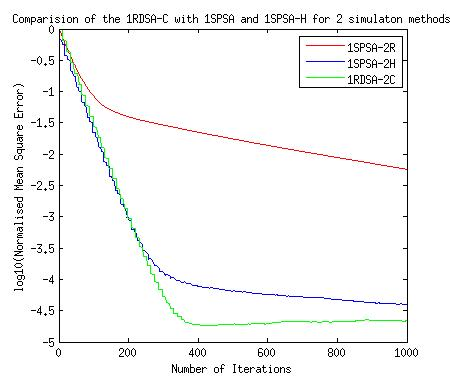
\includegraphics[width=8cm, height=7cm]{results_noise_quad.jpg}\label{fig:noise_quad}
% \end{figure}
% 
% \begin{figure}
% \caption{$\log_{10}(\text{NMSE})$vs No of iterations for fourth order objective 
% objective \eqref{eq:4thorder} with noise ($\sigma=0.01$) using 2 simulation methods.}
% 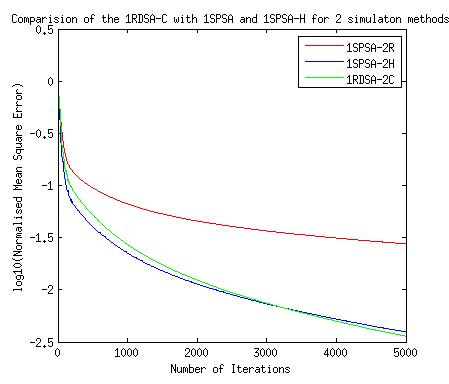
\includegraphics[width=8cm, height=7cm]{results_noise_fourthorder.jpg}\label{fig:noise_4thorder}
% \end{figure}
% 
% \begin{figure}
% \caption{$\log_{10}(\text{NMSE})$vs No of iterations for quadratic order objective 
% objective \eqref{eq:quadratic} with noise ($\sigma=0.01$) using 1 simulation methods.}
% 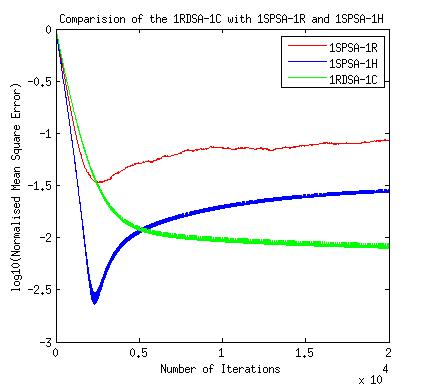
\includegraphics[width=8cm, height=7cm]{results_noise_1sim_quad.jpg}\label{fig:noise_quad_1sim}
% \end{figure}
% 
% \begin{figure}
% \caption{$\log_{10}(\text{NMSE})$vs No of iterations for fourth order objective 
% objective \eqref{eq:4thorder} with noise ($\sigma=0.01$) using 1 simulation methods.}
% 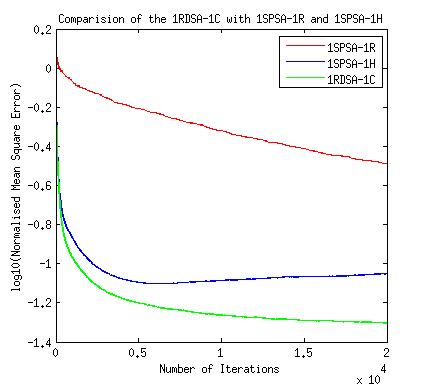
\includegraphics[width=8cm, height=7cm]{results_noise_1sim_fourthorder.jpg}\label{fig:noise_4thorder_1sim}
% \end{figure}

% Tables \ref{tab:NMSE-quadratic}--\ref{tab:NMSE-fourthorder} present the 
% normalized mean square values observed for the three algorithms - 1SPSA-2R, 1SPSA-2H and 
% 1RDSA-2C for the quadratic and fourth-order loss functions respectively.
% Tables \ref{tab:NMSE-quadratic-1sim}--\ref{tab:NMSE-fourthorder-1sim} present 
% the NMSE values observed for the three algorithms - 1SPSA-1R, 1SPSA-1H  and 1SPSA-1C
% with quadratic and fourth order loss functions respectively. 
% The results  in Table \ref{tab:NMSE-quadratic} are obtained after $2000$ simulations and
% the results in Table \ref{tab:NMSE-fourthorder} are obtained after $10000$ simulations.
% The results in Tables --\ref{tab:NMSE-quadratic-1sim}--\ref{tab:NMSE-fourthorder-1sim} are 
% obtained after running the one simulation algorithms with a budget of $20000$ simulations. 

% Figures \ref{fig:noise_quad} and \ref{fig:noise_4thorder} show plots of $\log_{10}\text{(NMSE)}$ as
% a function of number of iterations with quadratic and fourth-order loss objectives respectively,
% with $\sigma=0.01$, when 2-simulation methods are used. 
% 
% 
% Figures \ref{fig:noise_quad_1sim} and \ref{fig:noise_4thorder_1sim} plot the 
% $\log_{10}\text{(NMSE)}$ as a function of the iterations with quadratic and fourth-order loss 
% objectives respectively, with $\sigma=0.01$, when 1-simulation methods are used. 

% From the results in Tables \ref{tab:NMSE-quadratic},\ref{tab:NMSE-fourthorder},
% \ref{tab:NMSE-quadratic-1sim},\ref{tab:NMSE-fourthorder-1sim} and 
% plots \ref{fig:noise_quad},\ref{fig:noise_4thorder},\ref{fig:noise_quad_1sim}, 
% \ref{fig:noise_4thorder_1sim}, we make the following observations:

From the results in Tables \ref{tab:NMSE-quadratic},\ref{tab:NMSE-fourthorder},
\ref{tab:NMSE-quadratic-1sim} and \ref{tab:NMSE-fourthorder-1sim} 
we make the following observations:

\textit{\textbf{Observation1}} In the case of two simulation algorithms, 
1RDSA-2C is slightly better than 1SPSA-2H, while both of them outperform 1SPSA-2R.

\textit{\textbf{Observation2}} In the case of one simulation algorithms, 
1RDSA-1C is better than both 1SPSA-1H and 1SPSA-1R.


\section{CONCLUSIONS}
\label{sec:conclusions}
We presented a novel construction of deterministic perturbations for 
1RDSA-2R and 1RDSA-1R algorithms and showed that the resulting algorithms 
1RDSA-2C and 1RDSA-1C are provably convergent. 
The advantage with our deterministic perturbation construction is that the
same set of perturbations can be used for both two simulation
and one simulation variants. These perturbations also have a smaller cycle length compared to 
Hadmard matrix based perturbations. Numerical experiments demonstrated that 1RDSA-2C (1RDSA-1C) outperforms 
1SPSA-2R (1SPSA-1R) and 1SPSA-2H (1SPSA-1H).
As future work, it would be interesting to derive similar methods in the context of 
2RDSA. A challenging future direction would be to derive weak convergence results when
deterministic perturbations are used.
\bibliography{reference}
\bibliographystyle{IEEEtran}
\end{document}
